%chapappendix.tex
%
%Appendices are written like the body of the paper using
%\verb+\chapter+.
%\LaTeX\ numbers them with capital letters.
%If there is only one appendix, 
%then use \verb+\oneappendix+ instead of \verb+\chapter+
%so that the table of contents is properly formatted.
%
%The MSU library requires that each appendix have a 
%separator page.  The following lines in 
%{\tt examplethesis.tex} achieve this.
%
%\newspacing{\singlespacing}\begin{verbatim}
%%MSU library requires title page for each appendix
%\renewcommand{\appendixname}{\vspace*{2.5in}Appendix} 
%%for appendix title page
%\oneappendix{An Example} %for a single appendix
%%\chapter{An Appendix Title} 
%%alternative for each of multiple appendices
%\newpage %end of appendix title page
%\input{exappendix} %content of appendix
%\end{verbatim}\newspacing{\defaultspacing}
%
%The \verb+\vspace*+ command provides 
%the proper layout of the title page.
%This example has only one appendix.  
%Therefore, the
%\verb+\oneappendix+ command is used.
%The \verb+\newpage+ command forces a page break
%after the title page.
%If you have multiple appendices, then
%use the \verb+\chapter+ command for each appendix
%instead of \verb+\oneappendix+,
%and put \verb+\newpage+ after each \verb+\chapter+ command.

\Section{Transparency with Respect to Hydrogen}%
\label{Transparency with respect to Hydrogen}
Transparency of kaon with respect to free-nucleon cross section for three kinematics for all the targets is shown in \Tableref{t_2}. We used hydrogen cross section as the free-nucleon cross section. The total uncertainty has been taken as the quadrature sum of the statistical and systematic uncertainty. The different targets are shown by different colors as: BLACK- $LD_2$, RED- carbon, GREEN- copper and BLUE- gold for three different kinematics ($Q^2$= 1.1, 2.2 and 3.0 $(\mathrm{GeV/c})^2$). In \figureref{transp1}, the inner bar shows the statistical uncertainty and outer bar shows the systematic uncertainty and total uncertainty as quadrature sum these two.

\begin{figure}[!tbp]
  \centering
  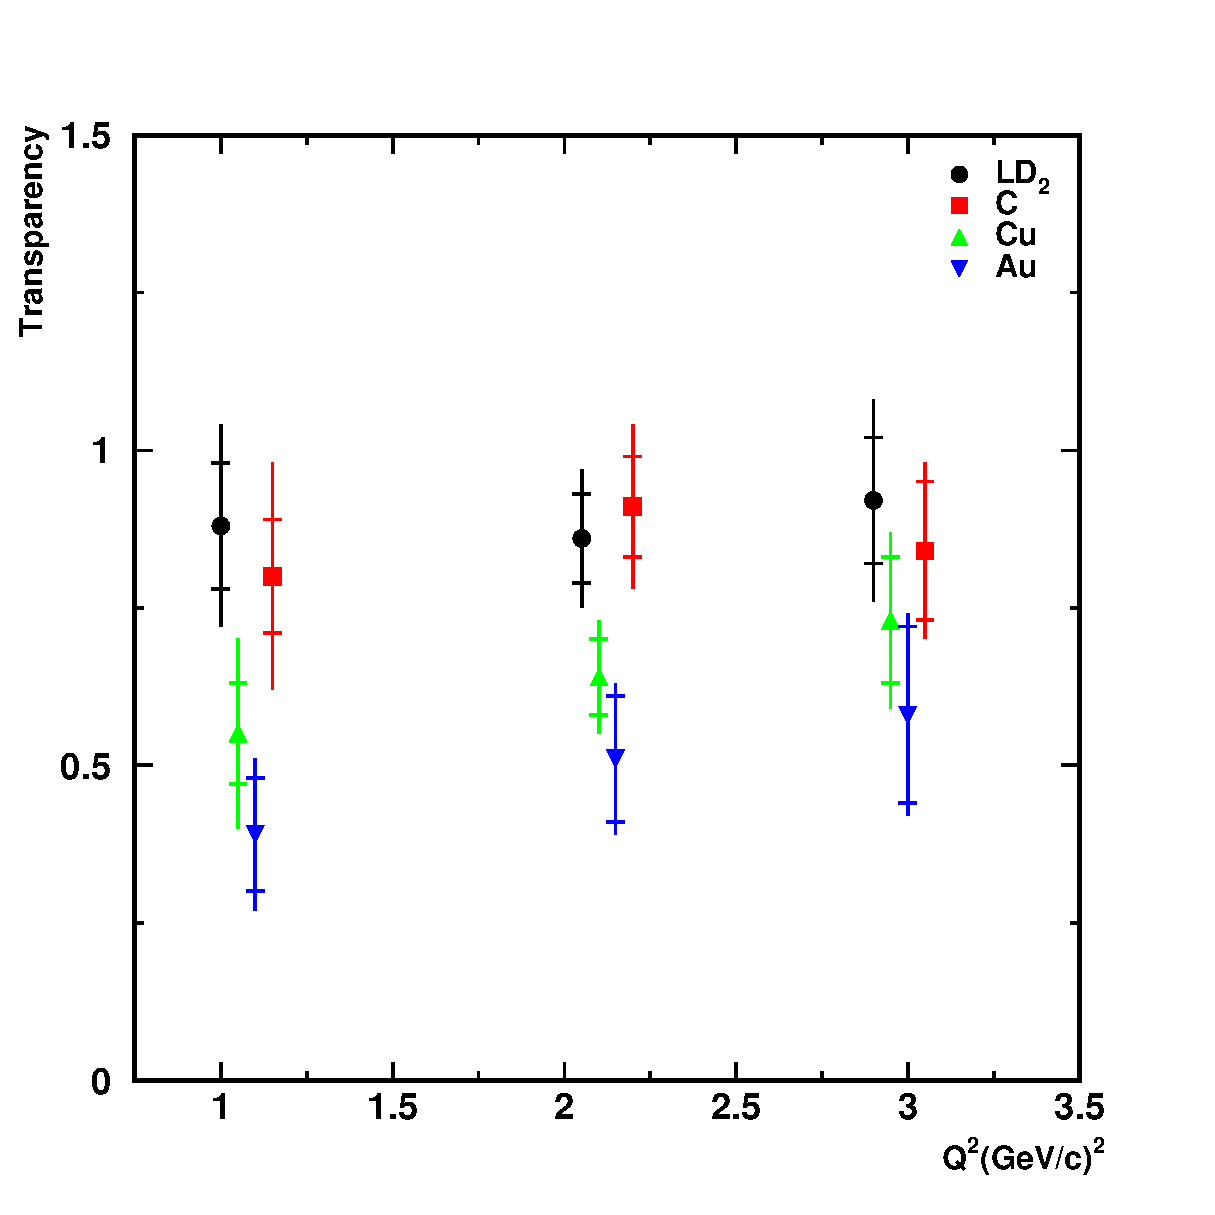
\includegraphics[width=0.8\columnwidth]{transp1}
  \caption[Nuclear transparency with respect to $H_2$ target.]{\label{fig:transp1}Nuclear transparency with respect to $H_2$ target.\\\\ Copper, carbon and $LD_2$ are shifted by -0.05, 0.05 and -0.10 $(\mathrm{GeV/c})^2$ in $Q^2$, respectively, for convenience.}
\end{figure}
%\setlength{\figwidth}{0.8\linewidth}
%\Figure{transp1}{\figwidth}{Nuclear transparency for different targets. Copper, carbon and $LD_2$ are shifted by -0.05, 0.05 and -0.10 $(\mathrm{GeV/c})^2$ in $Q^2$, respectively, for convenience.}

\Table{t_1}{Cross section for hydrogen for different $Q^2$ for kaons.}

%\begin{table}
%  \caption[T and $\sigma_{eff}$ for different targets with respect to $H_2$.]{\label{tab:t_2}T and $\sigma_{eff}$ for different targets with respect to $H_2$.\\\\ Different kinematic settings for kaons with respect to the free space cross section are shown here.}
%\begin{center}
\begin{tabular}{||c|c|c|c|c|c|c||}\hline
 Target & $Q^2$ & Cross section & Transparency & Statistical & Systematic & Total \\
 & $(GeV/c)^2$ & (mb) & & error($\%$)& error($\%$)&error($\%$) \\\hline
$LD_2$ & 1.1 & 8.38 & 0.88 & 10.30 & 12.34 & 16.07\\
Carbon & 1.1 & 7.57 & 0.80 & 09.31 & 16.11 & 18.61\\
Copper & 1.1 & 5.17 & 0.55 & 07.85 & 12.69 & 14.92\\
Gold   & 1.1 & 3.64 & 0.39 & 09.03 & 07.13 & 11.51\\\hline
$LD_2$ & 2.2 & 7.53 & 0.86 & 07.51 & 07.48 & 10.61\\
Carbon & 2.2 & 8.01 & 0.91 & 07.58 & 10.03 & 12.57\\
Copper & 2.2 & 5.60 & 0.64 & 06.45 & 06.43 & 09.11\\
Gold   & 2.2 & 4.49 & 0.51 & 09.93 & 06.40 & 11.82\\\hline
$LD_2$ & 3.0 & 8.55 & 0.92 & 10.22 & 12.06 & 15.81\\
Carbon & 3.0 & 7.76 & 0.84 & 11.49 & 08.10 & 14.06\\
Copper & 3.0 & 6.75 & 0.73 & 10.24 & 09.33 & 13.85\\
Gold   & 3.0 & 5.42 & 0.58 & 13.91 & 08.22 & 16.16\\\hline
\end{tabular}
\end{center}
%\end{table}
\Table{t_2}{T and $\sigma_{eff}$ for different targets with respect to $H_2$.}

\Table{t_3}{Cross section for deuterium for different $Q^2$ for kaons.}